%% -*- mode: poly-noweb+R; ess-indent-level: 2; -*-
\chapter{Az \code{EXCEL} oldal felhasználói szemmel}
\label{chap:3}

Az \code{Rxls} \code{R} csomagban három \code{EXCEL} munkafüzet van.
\begin{description}
\item[{\code{R.xls}}] Ez egy Office XP kompatibilis munkafüzet. Ez az
  amit az alkalmazások ténylegesen használnak. Ebben van megoldva a
  \code{R} példány megkeresése és az összeköttetés létrehozása,
  valamint néhány olyan rutin is ami a számoló munkafüzetekben
  szükséges lehet: file és mappa választás, valamint ACCESS tábla választás.
\item[\code{Rdev.xlam}] Ez a munkafüzet egy bővítmény, ami a számoló
  munkafüzetek létrehozásához ad segítséget.
\item[\code{Calc.xltm}] A számoló munkafüzetek templateje.
\end{description}

\section{Az \code{Rdev.xlam} bővítmény}
\label{sec:3.1}

\subsection{\code{Rdev.xlam}}
Ebbe a munkafüzetbe gyűjtöttem azokat a rutinokat, melyek csak a
fejlesztéshez szükségesek. Ezek munkalap védelem be és kikapcsolása, \code{R}
kód elrejtése és felfedése, valamint a munkafüzet véglegesítése. A
véglegesítés a munkalapok védelmének bekapcsolását, a kódot tartalmazó
munkalapok elrejtését jelenti. Ennek során a védett munkalapokon a
felhasználó által kitöltendő mezők zárolása feloldódik. Az, hogy
melyik cella tartozik ebbe a csoportba a kitöltés színe határozza meg.

A tényleges számolást végző \code{R} rutinokat talán  legegyszerűbb magában
a számoló munkafüzetben tárolni. Másik lehetőség lehetne, hogy a
feladatra szabott \code{R} csomagot készítünk és azt telepítjük a felhasználó gépére.

Az \code{R} kódot tehát \code{EXCEL} munkalapon szeretnénk tárolni. Szerkeszteni,
tesztelni viszont 
nem itt célszerű. A követendő eljárás az lehet, hogy pl. \code{Rstudio}-ban
fejlesztünk és a kész kódot bemásoljuk a munkafüzetbe. Az ilyen
\code{R} kódot tartalmazó munkalapokat a továbbiakban 
\code{R kódlap}nak fogom nevezni.

Ez a bővítmény számos új menüpontot definiál. Az \code{EXCEL} újabb, \code{RIBBON}
felületet használó, változataiban létrehoz egy \code{Rxls development}
tabot, a korábbi változatokban pedig 
ugyanilyen névvel egy menüpontot, az \code{EXCEL} fő menüsorában. Emellett a
cell menü is kiegészül néhány ponttal és a munkalap fülek menüje is kap
egy új menüpontot. 

\subsection{Az \code{Rxls development} fül elemei}
A \code{Rxls development} fülön lévő parancsok elérhetőek a
\code{Bővítmények} fül alatti %\code{R} és \code{Rxls development}
menüpontokból is. Az \code{EXCEL} korábbi, nem a \code{RIBBON}
felületet használó változataiban pedig a menüsorban bővül ki két ponttal. 
\begin{figure}[h]
  \centering
  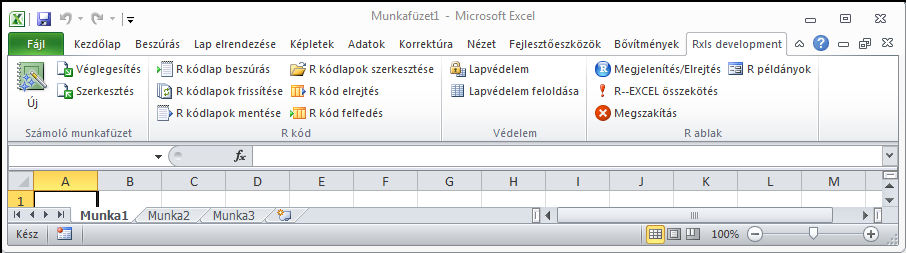
\includegraphics{images/Rxls_development_menu}
  \caption{Az \code{'Rxls development'} menü.}
  \label{fig:3.1}
\end{figure}

\subsubsection{\code{Számoló munkafüzet} csoport}
Itt csak három gomb található, \code{Új}, \code{Véglegesítés}
ill. \code{Szerkesztés} névvel.
Az \code{Új} gomb, létrehoz egy új számoló munkafüzetet. Ez a \code{Calc.xltm}
template egy másolata lesz. Célszerű rögtön elmenteni a létrehozás
után valamelyik makróbarát formátumba. Ennek oka, hogy néhány munkalapfüggvény 
(\code{INFO}, \code{CELLA}) másként viselkedik mentett munkafüzetben, mint
mentetlenben.
%munkafüzetbe kell
%menteni.
% A létrehozás során rögtön el is
% mentjük. Ennek oka, hogy néhány munkalapfüggvény 
% (\code{INFO}, \code{CELLA}) másként viselkedik mentett munkafüzetben, mint
% mentetlenben. A számoló munkafüzet \code{xls} kiterjesztésű, azaz
% korábbi OFFICE változatokban is megnyitható.

A \code{Véglegesítés} menüparancs hatására a számoló munkafüzet \code{R
  kódlap}jai rejtetté válnak, hasonlóan az \code{Adatok} munkalap
\code{\# R nevek \#} oszlopához. Valamennyi cella zárolt lesz 
kivéve azokat, amelyek színe megegyezik a \code{customvalue} színnel. Ez a
szín \code{R kód} munkalap 
\code{colortable} tartományából derül ki. A tartomány elemei színes
cellák, a cella értéke a szín neve. Végül a kapott munkafüzetet elmentjük.

A \code{Szerkesztés} a \code{Véglegesítés} ellentéte. A
munkalapvédelmet kikapcsolja, a rejtett munkalapokat és oszlopokat
láthatóvá teszi.

\subsubsection{\code{R kód} csoport} 
Az első oszlopban az \code{R kódlap}ok kezelésére szolgáló parancsok
vannak. Beszúrás, frissítés és mentés. Frissítés és mentés esetén elő
fordulhat a korábbi változatok felülírása. Ilyen esetben 
egy felugró ablakban meg kell erősíteni a szándékot.

A második oszlop elemeinek segítségével az \code{R kód} nevű munkalapokat
elrejthetjük, ill. ha további szerkesztésre van szükség felfedhetjük
és megnyíthatjuk a \code{.R} kiterjesztéshez asszociált szerkesztővel
(szerencsés esetben ez az \code{Rstudio}).

\subsubsection{\code{Védelem} csoport}
Lapvédelem be- ill. kikapcsolása. Ez a két rutin (a \code{Véglegesítés}-sel
ellentétben) nem módosítja a cellák zárolását. 

\subsubsection{\code{R ablak} csoport}
Ez a csoport az \code{R.xls} munkafüzetben definiált rutinokat teszi elérhetővé.
\begin{description}
\item[\code{Megjelenítés/Elrejtés}] Ha nincs aktív \code{R} példány,
  akkor a futó \code{R}  példányok közül választhat egyet a
  felhasználó. Ha nincs futó \code{R}, 
  akkor elindítunk egyet, ha pontosan egy \code{R} példány fut, akkor azt
  fogjuk használni. A gomb megnyomása után a kiválasztott \code{R} példány
  aktív lesz és az ablaka látható. 
  
  Ha már van aktív \code{R} példányunk,
  akkor a gomb megnyomása után annak ablaka rejtetté válik. Továbbra
  is használható lesz, de az asztalon nem lesz nyoma.

\item[\code{R--EXCEL összekötés}] Az aktív \code{R} példányban
  létrehozza a \code{THISXL} 
  változót, ami az \code{EXCEL} példányra mutató \code{COMObject} (Ez
  tulajdonképpen  az \code{EXCEL} Visual Basic \code{Application}
  változójának értéke). 

  Ha nincs aktív \code{R} példány, akkor létrehoz egyet, hasonlóan a
  \code{Megjelenítés}hez, de az így 
  létrehozott \code{R} példány ablaka alapértelmezésben háttérben marad.
  
\item[\code{Megszakítás}] Az \code{R} oldalon folyó számolást próbálja
  megszakítani, az aktív \code{R} példány konzoljába küldött
  \code{ESCAPE} karakterrel.  
\end{description}

\subsection{\code{Cella} menü}

\begin{figure}[h]
  \centering
  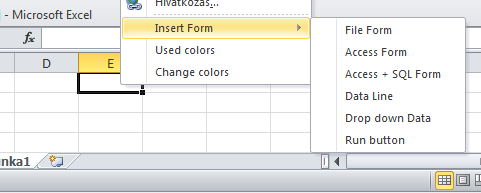
\includegraphics[width=20em]{images/cella-menu}
  \caption{A cella menü új elemei.}
  \label{fig:3.2}
\end{figure}

\begin{description}
\item[\code{Insert Form}] Ez egy menüt kínál fel, amiben a számoló
  munkafüzetek szokásos elemei találhatóak: 

  \begin{description}
  \item[\code{File form}] Egy három sorból és négy oszlopból álló tartományt
    tölt ki az aktív munkalapon, melynek bal felső sarka az aktív
    cella. A tartomány első sora címsor, a  második sorban a
    könyvtár, a harmadikban a file neve adható meg. A második és
    harmadik sor felhasználói mezőjében található gombok hatására az
    \code{EXCEL} file választó dialógja jelenik meg, így nem kell az
    elérési utat és a file nevet kézzel beírni.  A file típusát egy
    felugró inputboxban adhatjuk meg. Valójában itt a file filtert
    kell megadni \code{leírás,*.kiterjesztés} alakban. Az \code{EXCEL},
    \code{.RData}, és \code{.R} 
    file típusokat a legördülő menüből is ki lehet választani. Ha
    üresen hagyjuk az inputboxot, akkor  tetszőleges file típust
    választhat majd a felhasználó.  

    Ha egy már kitöltött \code{File form} file típusát, utólag
    módosítani akarjuk, akkor azt a gombhoz rendelt makróban tehetjük meg.
  \item[\code{Access form}] Hasonló a \code{File form}-hoz, azonban
    egyel több sort tölt ki a munkalapon.  Az utolsó 
    sorban az \code{ACCESS} adatbázis táblái közül lehet választani.  
  \item[\code{Access + SQL form}] Volt olyan korábbi munka, ahol
    felmerült, hogy nem csak 
    \code{ACCESS} adatbázisból, hanem más \code{SQL} lekérdezést
    használó rendszerből is lehessen adatot lekérdezni. Ez az űrlap
    erre szolgál. A bal felső sarkában van egy gomb, ami két lehetőség között
    kapcsolgat. Így csak az egyik opció látható. Az \code{ACCESS form}hoz 
    képest van egy plusz sor ami az \code{ACCESS} lekérdezés \code{where}
    klauzulájának megadására szolgál. Ha átkapcsolunk \code{SQL} módra, akkor
    a kapcsolat létrehozásához szükséges \code{DSN} karakterláncot és
    az \code{SQL} 
    parancsot kell megadni. Mivel csak a látható sorokban lévő adatok
    kerülnek át az \code{R} oldalra, az \code{R} program el tudja
    dönteni, milyen 
    adatbázist kell használnia. Pl. ha az \code{SQL} parancs \code{R} neve
    \code{lekerdezes1.SQL}, akkor a következő kód részlet 
    \begin{Rnw}
<<eval=FALSE,prompt=FALSE>>=
if(exists("lekerdezes1.SQL")){
    ## kód az SQL ághoz
}else{
    ## kód az ACCESS ághoz
}
@
    \end{Rnw}
 % if
 %    (exists("lekerdezes1.SQL")) { ## kód az SQL ághoz } else { ## kód
 %      az ACCESS ághoz }
    választ a kétféle adatforrás közül. Mindez
    csak akkor működik megbízhatóan, ha  olyan nevet adunk, ami nem
    létezik a globális környezetben. Nem célszerű pl. az \code{x} vagy
    \code{i} használata. Egy másik 
    gond az lehet, hogy ha mindkét adatforrást szeretnénk egy-egy
    futás erejéig kipróbálni. Ilyenkor az \code{XLdata} függvény \code{rmHidden}
    argumentumát is igazra kell állítani, lásd a \ref{sec:7.1} szakaszt. Ezt az
    \code{R kód} munkalap \code{\$K\$21} mezőjében célszerű megtenni. A képletet
    célszerű átírni a következő módon:
\begin{VBAframe}
="XLdata(1, 4, rmHidden=TRUE, range='_Rdata')"
\end{VBAframe}
    Ha egy függvényen belül kell ellenőrizni, hogy létezik-e a
    paraméterként átadott  érték, akkor a 
    használhatjuk a \code{getFromDB} függvényt mintaként: 
    \begin{Rnw}
<<>>=
getFromDB
@      
    \end{Rnw}
% > getFromDB
%     function (dir, file, table, where = "", dsn, sql) { if
%       (!inherits(try(dsn, silent = TRUE), "try-error")) { ODBC.get(dsn
%         = dsn, sql = sql) } else { ACCESS.get(dir = dir, file = file,
%         table = table, where = where) } } <environment:
%     namespace:Rxls> 
    Ekkor, ha az \code{Adatok} munkalapon a \code{DSN}, \code{SQL} sorok
    el vannak rejtve és az \code{XLdata}, \code{rmHidden} paramétere
    \code{TRUE}, akkor a 
    függvény az \code{ACCESS} ágon ellenkező esetben pedig az
    \code{SQL} ágon fog 
    végig menni. A módszer az \code{R} \code{try} függvényét használja, ami
    megpróbálja kiértékelni az első argumentumát (ez jelen esetben a
    \code{dsn} argumentum). Ha a kiértékelés hiba nélkül megtörténik, akkor
    a kiértékelés eredményét kapjuk, ha hiba történt, akkor egy hiba
    (\code{try-error} osztályú) objektumot.  Az \code{inherit}
    függvény ellenőrzi, 
    hogy egy adott érték osztályai között szerepel-e  a megadott
    név. \code{R}-ben minden változónak van osztálya, vagy explicit (a
    \code{class} 
    attribútum értéke) vagy implicit módon (ezek az alaptípusok,
    pl. \code{numeric}, stb.) 

    Az \code{ACCESS.get} és \code{ODBC.get} függvények
    definiálva van az \code{Rxls} csomagban. Az \code{ODBC.get} rutint
    nem tudtam  tesztelni az érdekes esetben, amikor \code{Oracle}
    rendszerhez akarunk 
    csatlakozni.  
\item[\code{Data Line}] A kijelölt tartomány minden sorát kitölti
    egy-egy adat sorral. Használatával már találkoztunk az \ref{sec:1.3}
    részben.  
  \item[\code{Drop down data}] Ha egy adat sorban csak néhány lehetőség
    közül választhat a felhasználó, akkor célszerű azt egy legördülő
    menüben felkínálni számára. Erre szolgál ez a menüpont.
    
    Hozzunk létre egy adat sort a \code{Data Line} beillesztése parancs
    segítségével, majd a felhasználói beállításnak fenntartott mezőbe
    írjuk be a lehetőségeket pontosvesszővel
    elválasztva. Ezután jelöljük ki a cellát és klikkeljünk a jobb
    egérgombra, majd válasszuk ki a \code{Drop down data} menüpontot. Ekkor
    az \code{R kód} munkalapon létrejön a választék lista az
    \code{\$A:\$A} oszlop 
    végén és a legördülő űrlap alatti cella képlete kitöltődik.

    Több cellát is kijelölhetünk. Ilyenkor mindegyik kijelölt cellába
    egy legördülő menü kerül a cella tartalma alapján.  Ha a
    kijelölt cella üres, akkor a választéklista hosszát kell megadni
    egy felugró input mezőben. A lista elemeit később az \code{R kód}
    munkafüzetben adhatjuk meg.

   
    {%\tracingall
      \Aref{sec:1.3}} részben már
    láthattunk példát a \code{Drop down data} alkalmazására.
  \item[\code{Run button}] Erre  akkor lehet szükség, ha a fő számolás
    mellett valamilyen rész 
    feladatot szeretnénk külön is végrehajthatóvá tenni.  A kijelölt
    tartomány fölé beilleszt egy gombot \code{Számolás indítása} szöveggel. A
    gomb alatti cellák szövegét küldi át az \code{R}-nek végrehajtásra. Ez
    pl. lehet
\begin{VBAframe}
="XLsource(<R kódlap neve>, wbname=.wbname)"
\end{VBAframe}
    A \code{.wbname} \code{R} változó értéke 
    %a futási környezetbe  név értéke az \code{R kódlap} munkalapon van megadva és az
    aktuális munkafüzet neve a megfelelő formában. A szükséges adatok
    átadását célszerű az \code{R  kódlapon} elvégezni, pl. az \code{XLdata}
    függvény használatával.
  \end{description}
\item[\code{Used colors, Change colors}] Kigyűjti,
  ill. átállítja a munkafüzetben használt színeket. Részletesen lásd
  \aref{sec:3.3} szakaszban.
\end{description}
\subsubsection{Munkalap fül}

 Itt is elérhető az \code{R kódlap} beszúrás parancs számoló
 munkafüzeteken belül.  \code{R kódlap}ok fülén megjelenik még a
 szerkesztés és frissítés parancs is.

\begin{figure}[h]
  \centering
  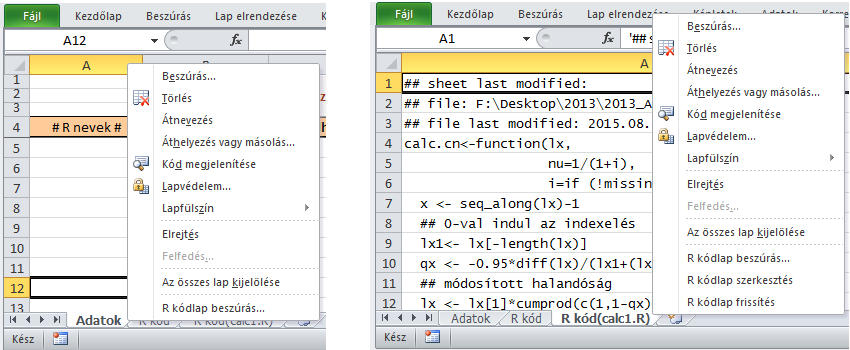
\includegraphics{images/ply_menu}
  \caption{A munkalap fül menü új elemei.}
  \label{fig:3.2a}
\end{figure}

\section{Melyik \code{R} példányt használjuk?}
\label{sec:3.2}

\code{R} példány három formában fordulhat elő: terminál ablakban indított \code{R}, \code{RGui}, ill. az \code{Rstudio}
\code{rsession} szála. Mindegyiknek lehet 32–bites ill. 64–bites
változata. 
%Mivel a \code{com} csomag csak  a 32–bites változaton működik,
%\code{EXCEL}-ből csak ezt tudjuk használni. 
Az \code{RGui} két változatban
fordulhat elő \code{MDI} (sok kis ablak egy nagy ablakon belül)
ill. \code{SDI} (sok egymástól független ablak). Az \code{Rxls}
mindegyik változatot tudja kezelni, de ha nincs futó példány, akkor
mindig az \code{RGui}-t indítja el, \code{SDI} módban. A felhasználói beállítások (esetleges \code{Rprofile} file tartalma)
nem érvényesülnek, mert a programot \code{--vanilla} opcióval
indítjuk.

A legegyszerűbb eset, az amikor nincs futó \code{R} példány, vagy
pontosan egy van. Ha nincs 
futó \code{R} példány, akkor elindítunk egy újat és egyből betöltjük
az \code{Rxls}, \code{comproxy} és \code{com} csomagokat.

Ha pontosan egy futó \code{R} példány van, akkor azt próbáljuk
használni. Ezt lehetne finomítani, mert az általunk indított \code{R}
példányokban feljegyezzük az \code{EXCEL} alkalmazás azonosítóját 
(\code{hinstance}) a \code{.startingapp} változóban. Így ha el is
veszítettük a kapcsolatot valamilyen 
oknál fogva le tudjuk ellenőrizni, hogy a futó \code{R} példányt mi
indítottuk el vagy sem. 

Ha több \code{R} példány fut éppen, akkor a felhasználónak kell
választania egy felugró ablakban. Ekkor is lehetőség van új példányt
indítani. 
\begin{figure}[h]
  \centering
  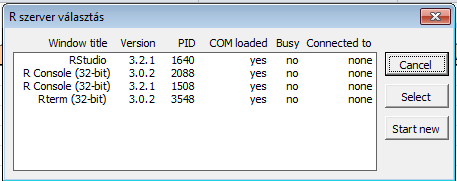
\includegraphics[width=22em]{images/rselect}
  \caption{R szerver választó dialóg}
  \label{fig:3.3}
\end{figure}

A választó dialógban megjelenő információk:
\begin{description}
\item[\code{windowtitle}, \code{PID}] Az \code{R} ablak címsora, ill. az
adott \code{R} példány \code{process id}-je. 
\item[\code{COM loaded}] Azt mutatja, hogy a com csomag be van-e töltve.
\item[\code{busy}] Ha a \code{com} csomag be van töltve, akkor le tudjuk
  kérdezni a \code{sys.nframe()} értéket. Ennek értéke 0, ha az
  \code{R} nem végez 
  számolást, és legalább 1 ha éppen függvény kiértékelés zajlik. Ha a
  \code{com} csomag nincs betöltve a mező értéke \code{???}.  
\item[\code{connectedTo}] Ha a \code{com}
  csomag be van töltve, akkor le tudjuk ellenőrizni, hogy létezik-e a
  \code{THISXL} változó az \code{R} oldalon és az a mi \code{EXCEL}
  példányunkra mutat-e? 
  Ez alapján meg tudjuk mondani, hogy az adott \code{R} példány a mi
  \code{EXCEL} 
  példányunkkal van összekötve, másikkal, vagy egyikkel sem.
\end{description}
Ha van rá igény a fenti lista esetleg kiegészíthető azzal is, hogy a
mi \code{EXCEL} példányunk indította-e el az adott \code{R} példányt.

\section{Színek}
\label{sec:3.3}

A számoló munkafüzetek színesek. Számomra segítség, ha látom, hol
vannak a munkafüzeten adatok, melyek azok a mezők, amiket ki kell vagy
ki lehet tölteni, melyek a feliratok, számolt mezők, stb.. 
A színeket az Office XP által kínált skálából választottam annak idején, és
ezek a színek maradtak a mostani változatban is. Ugyanakkor az újabb
Office változatokban már nem csak egy limitált színsorból lehet
választani, hanem a teljes szín skála használható. 

Ha az \code{Rdev.xlam} munkafüzet be van töltve, akkor a \code{cella}
  menü kiegészül két menüponttal, \code{Used colors} és \code{Change
colors}. Mindkét parancs a kijelölt tartománnyal dolgozik. A
\code{Used colors} a kijelölt tartomány első oszlopát kitölti a
munkafüzetben használt színekkel. A 
\code{Change colors} esetében a kijelölésnek két oszlopot kell
tartalmaznia. Az első oszlop színeit 
a második oszlopban mellette található színre cseréli az egész
munkafüzetben.

A számoló munkafüzetek \code{R kód} munkalapján van egy \code{colortable}
nevű tartomány. Ennek első oszlopát nem érdemes változtatni. Ha a
munkafüzetet átszíneztük, akkor új elem beszúrásakor ebből derül ki,
hogy milyen színeket használ a munkafüzet az alapértelmezett színek 
helyett. A második oszlopot viszont kedvünkre átszínezhetjük és a
\code{Change colors} menü paranccsal az egész munkafüzetet
átszínezhetjük. Itt arra érdemes figyelni, hogy a négy szín 
különböző maradjon, de legalább a felhasználói adatoknak fenntartott
mező színe eltérjen 
a többitől. Ugyanis a véglegesítés során ez alapján derül ki, hogy
mely mezők maradjanak szerkeszthetőek.


Ha egyes részeket manuálisan hozunk létre vagy színezünk át, akkor az
utolsó fázisban 
célszerű egységesíteni a színeket. Ezt a legegyszerűbben úgy tehetjük
meg, hogy létrehozunk ideiglenesen egy új munkalapot, arra kigyűjtjük
a használt színeket a \code{Used colors} paranccsal, a mellette levő
oszlopban egységesítünk és a \code{Change colors} paranccsal a színeket 
átállítjuk. Ezután az ideiglenes munkalap törölhető.

Ha valaki az alapértelmezett színeket meg akarja változtatni, akkor
azt a \code{Calc.xltm} template átszínezésével érheti el. 

\section{Számoló munkafüzetek és az \code{R.xls} file}
\label{sec:3.4}

Ha egy számoló munkafüzetet  olyan \code{EXCEL} példányba töltünk be,
amire a \code{Rdev.xlam} bővítmény nincs telepítve, akkor a következő
történik. Megnyitás után a \code{Workbook\_Open} 
szubrutin ellenőrzi, hogy az \code{R.xls}-re mutató hivatkozás
érvényes-e, ha nem megpróbálja 
javítani és szükség esetén a felhasználó instrukciókat kap a
teendőiről. A menüsor egy új 
ponttal egészül ki, ez az \code{R} menü, melyből az \code{R ablak megjelenítés/elrejtés}, \code{R<->EXCEL}
összekötés és \code{R megszakítás} parancsok érhetőek el. Ezek
működése azonos \aref{sec:3.1} szakasz 
\code{R ablak} részében leírttal. A \code{RIBBON} felületet használó újabb \code{EXCEL} változatokban az \code{R} menü a
\code{Bővítmények} fül alatt található.

\endinput

%%% Local Variables: 
%%% mode: latex
%%% TeX-master: "Rxls"
%%% End: 
